\documentclass[10pt,a4paper]{article}
\usepackage[english]{babel}
\usepackage[utf8]{inputenc}
\usepackage{amsmath}
\usepackage{amsfonts}
\usepackage{amssymb}
\usepackage{graphicx}
\usepackage{float}
\usepackage{url}

%link to documentation: 
%https://ackrep-doc.readthedocs.io/en/latest/devdoc/contributing_data.html

\begin{document}
	\part*{Model Documentation of the \\ Distillation Column} % MUST - Add Model Name 
	
	%%%%%%%%%%%%%%%%%%%%%% NOMENCLATURE %%%%%%%%%%%%%%%%%%%%%%%%%%%
	
	\section{Nomenclature} % MUST
	\subsection{Nomenclature for Model Equations} % MUST
	
	%variables for model equations
	\begin{tabular}{ll}
		$K_{R1}, T_{N1}$ & parameters of the first PI controller \\
		$K_{R2}, T_{N2}$ & parameters of the second PI controller \\
		$K_1, K_2, K_3, K_4, T_1$ & parameters of the model, equilibrium point \\
		$x_S$ & filling level\\
		$x_T$ & temperature on the bottom\\
		$z_{ii}$ & malfunctions for i = 1, 2 \\
		$fb_i$ & feedback for i = 1, 2 \\
		$w$ & supply of heat steam, equivalent to  $M_H$ \\
				
	\end{tabular}
	
	\subsection{Signal Flowchart}
	\begin{figure}[H]
		\centering
		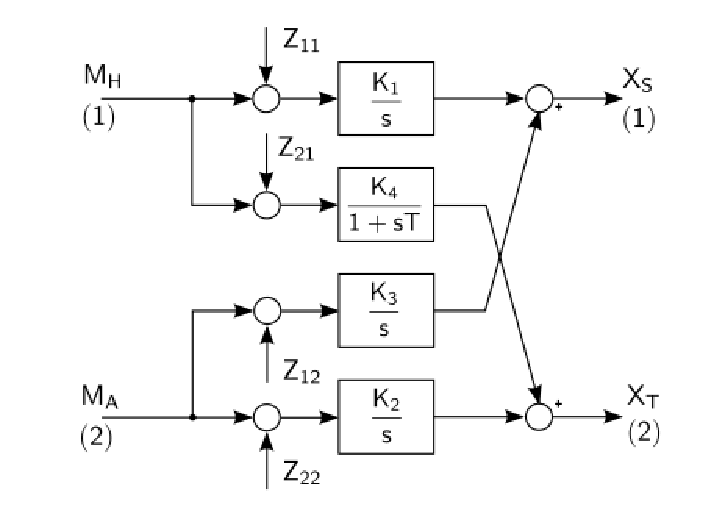
\includegraphics[width=70mm]{flowchart.pdf}
		\caption{Signal Flowchart}
	\end{figure}
	 
	
	%variables which are used additional to those in the model equations
	\begin{tabular}{ll}

	\end{tabular}
	
	%%%%%%%%%%%%%%%%%%%%%% MDOEL EQUATIONS %%%%%%%%%%%%%%%%%%%%%%%%%%%
	
	\section{Model Equations} % MUST
	
	State Vector and Input Vector:
	\begin{align*}
		\underline{x} &= (x_S \ x_T)^T &= (x_1 \ x_2)^T \\
		\underline{u} &= (fb_1 \ fb_2 \ w \ z_{11} \ z_{21} \ z_{12} \ z_{22})
					  &= (u_1 \ u_2 \ u_3 \ u_4 \ u_5 \ u_6 \ u_7)^T \\
	\end{align*}
	
	\noindent Transfer Functions:			
	\begin{subequations}
	\begin{align}
		G_{R_{11}} &= K_{R1}\left(1 + \frac{1}{sT_{N1}}\right) \\ 
		G_{R_{22}} &= K_{R2}\left(1 + \frac{1}{sT_{N1}}\right) \\
		G_{P_{11}} &= \frac{K_1}{s} \\
		G_{P_{12}} &= \frac{K_4}{1 + sT} \\
		G_{P_{21}} &= \frac{K_3}{s} \\
		G_{P_{22}} &= \frac{K_2}{s} 				
	\end{align}
	\end{subequations}

	%%%%%%%%%%%%%%%%%%%%%% PARAMETERS | OUTPUTS %%%%%%%%%%%%%%%%%%%%%%%%%%%
	\noindent
	Parameters: $K_{R1}, \, T_{N1}, \, K_{R2}, \, T_{N2}, \, T_1, \, K_1, \, K_2, \, K_3, \, K_4$ % variables with constant, predefined value
	\\
	Outputs: $x_1, \, x_2$ \\% MAY
	
	%%%%%%%%%%%%%%%%%%%%%% ASSUMPTIONS %%%%%%%%%%%%%%%%%%%%%%%%%%%

	%%%%%%%%%%%%%%%%%%%%%% EXEMPLARY PARAMETER VALUES %%%%%%%%%%%%%%%%%%%%%%%%%%%	
	
	\subsection{Exemplary parameter values}
	\begin{tabular}{cl}
\hline
  Symbol  & Value                                                                                                                                                                                \\
\hline
   $A$    & $\left[\begin{matrix}0.8189 & 0.0863 & 0.09 & 0.0813\\0.2524 & 1.0033 & 0.0313 & 0.2004\\-0.0545 & 0.0102 & 0.7901 & -0.258\\-0.1918 & -0.1034 & 0.1602 & 0.8604\end{matrix}\right]$ \\
   $B$    & $\left[\begin{matrix}0.0045 & 0.0044\\0.1001 & 0.01\\0.0003 & -0.0136\\-0.0051 & 0.0936\end{matrix}\right]$                                                                          \\
 $B_{1}$  & $\left[\begin{matrix}0.0045 & 0.0044\\0.1001 & 0.01\\0.0003 & -0.0136\\-0.0051 & 0.0936\end{matrix}\right]$                                                                          \\
 $C_{1}$  & $\left[\begin{matrix}1.0 & 0 & -1.0 & 0\\0 & 0 & 0 & 0\\0 & 0 & 0 & 0\end{matrix}\right]$                                                                                            \\
   $C$    & $\left[\begin{matrix}1.0 & 0 & 0 & 0\\0 & 0 & 1.0 & 0\end{matrix}\right]$                                                                                                            \\
 $D_{11}$ & $\left[\begin{matrix}0 & 0 & 0\\0 & 0 & 0\\0 & 0 & 0\end{matrix}\right]$                                                                                                             \\
 $D_{12}$ & $\left[\begin{matrix}0 & 0\\1.0 & 0\\0 & 1.0\end{matrix}\right]$                                                                                                                     \\
 $D_{21}$ & $\left[\begin{matrix}0 & 1.0 & 0\\0 & 0 & 1.0\end{matrix}\right]$                                                                                                                    \\
\hline
\end{tabular}

	%%%%%%%%%%%%%%%%%%%%%% DERIVATION & EXPLANATION %%%%%%%%%%%%%%%%%%%%%%%%%%%	
	
	\section{Derivation and Explanation} % SHOULD
	A rough analysis of the column behavior leads to the following approaches for the four subtransfer functions:
	\begin{align*}
		\frac{X_S}{M_H} = \frac{K_1}{s};\ \frac{X_T}{M_A} = \frac{K_2}{s};\ \frac{X_S}{M_A} = \frac{K_3}{s};\ \frac{X_T}{M_H} = \frac{K_4}{1 + sT}.
	\end{align*}
	$M_H$ is standing for the supply of the heat steam and $M_A$ represents the drain of the product. The system model is based on the signal flowchart.
	
	%%%%%%%%%%%%%%%%%%%%%% REFERENCES %%%%%%%%%%%%%%%%%%%%%%%%%%%
	
	\begin{thebibliography}{10}		
		\bibitem{But21}Institut für Regelungs- und Steuerungstheorie TU Dresden: \textit{Regelungstechnikpratikum, Praktikumsanleitung}, published in OPAL April 2022. \\
		(not publicly accessible)
		\bibitem{But21}Knoll, Carsten: \textit{Example2 : linear system consiting of various blocks}, Python Script published 2019. \\
		\url{https://github.com/TUD-RST/pyblocksim/blob/master/examples/example2.py}  
	\end{thebibliography}

\end{document}

